\section{Data}
\label{sec:data}

We explore the behavior of the metrics on mock data with well-understood systematics as well as realistic mock data from past classification challenges.

Data is in the form of catalogs of posterior probability vectors $p(m \mid d)$ over $M$ classes $m$ conditioned on the observed data $d$, where one class is designated ``other'' to encompass never-before-seen classes, and each probability vector is normalized to sum to unity.
Such probabilities are more valuable than point estimates, which we call deterministic metrics in this work, because of their versatility in application and encapsulation of observational and systematic error that may propagate through inference (Roberts+17).

\subsection{Mock classifier systematics}
\label{sec:mockdata}

The test cases of this section are introduced to confirm that our metric aligns with our intuitive understanding of what constitutes a good classifier, that it should not reward classifications suffering from the systematics that we find most concerning.

For each, we will address:
\begin{enumerate}
  \item What defines this systematic?
  \item When has this systematic cropped up in the literature?
  \item What are our expectations for metric behavior?
\end{enumerate}

\aim{Anita Bahmanyar will write the descriptions of and motivation for the confusion matrix-based systematics tests, as well as how the data is generated (what the underlying functions from the notebook are doing).}

\subsubsection{Agnostic classifier}
\label{sec:agnostic_data}

uniform probabilities across all classes

\begin{figure}
	\begin{center}
		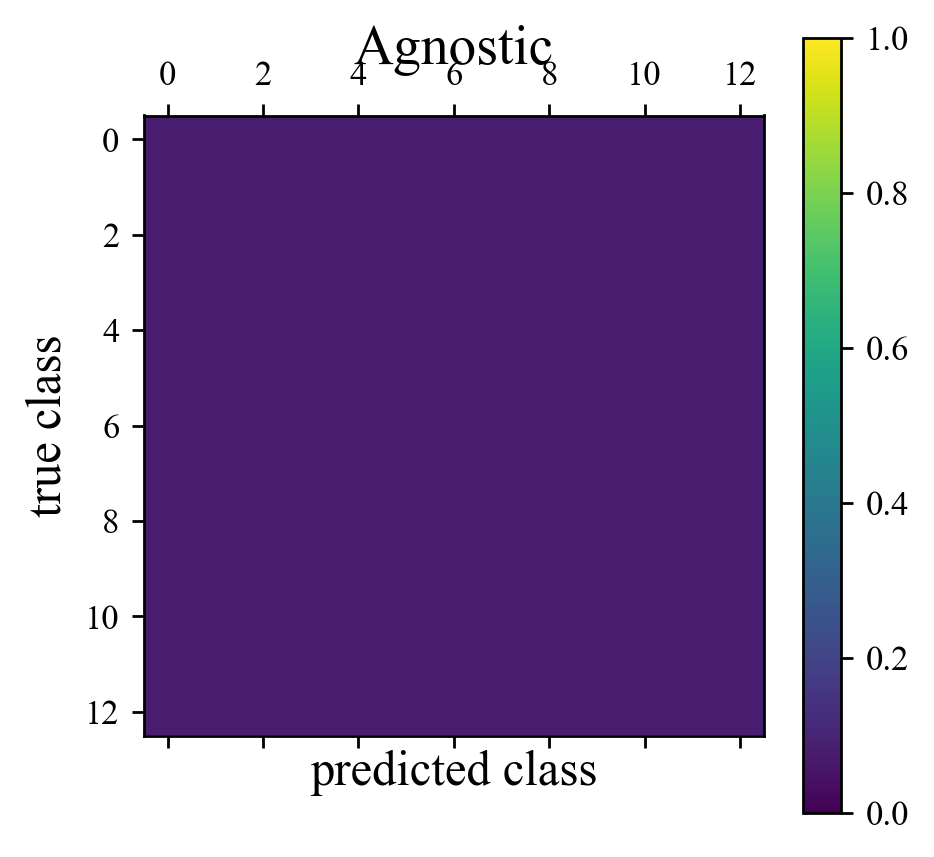
\includegraphics[width=0.45\textwidth]{./fig/Agnostic.png}\\
		\caption{}
		\label{fig:agnostic_data}
	\end{center}
\end{figure}

\subsubsection{Perfect classifier}
\label{sec:perfect_data}

perfectly accurate on all classes

\begin{figure}
	\begin{center}
		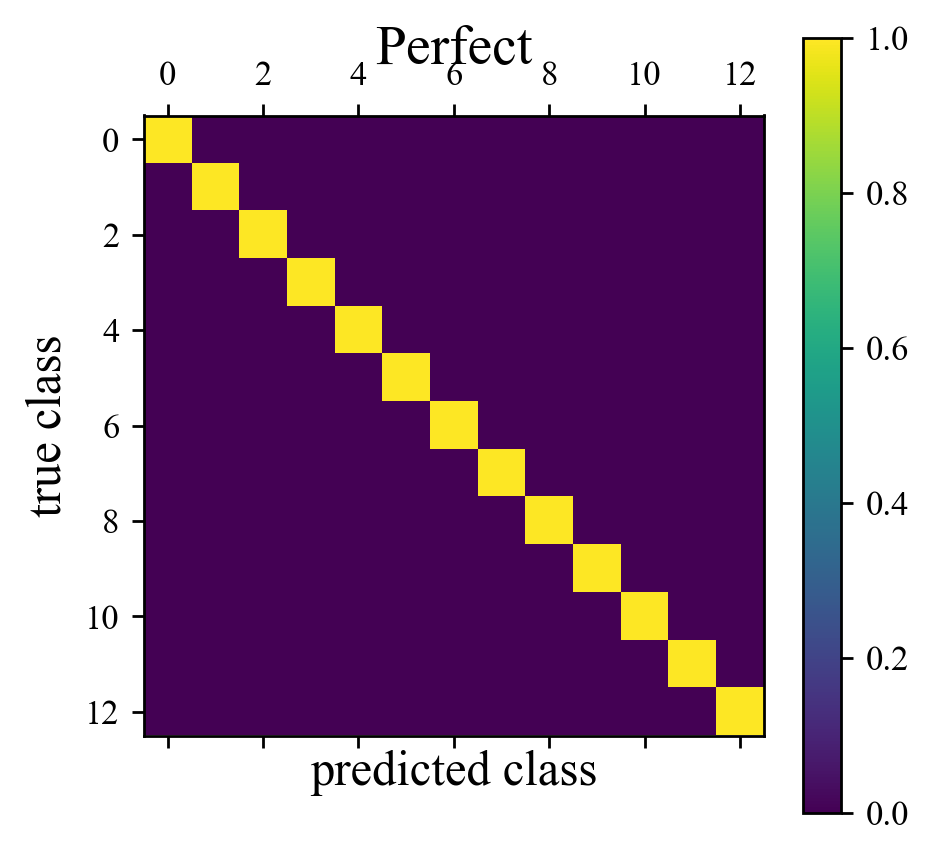
\includegraphics[width=0.45\textwidth]{./fig/Perfect.png}\\
		\caption{}
		\label{fig:perfect_data}
	\end{center}
\end{figure}

\subsubsection{Almost perfect classifier}
\label{sec:almost_data}

a slight perturbation of the perfect classifier

\begin{figure}
	\begin{center}
		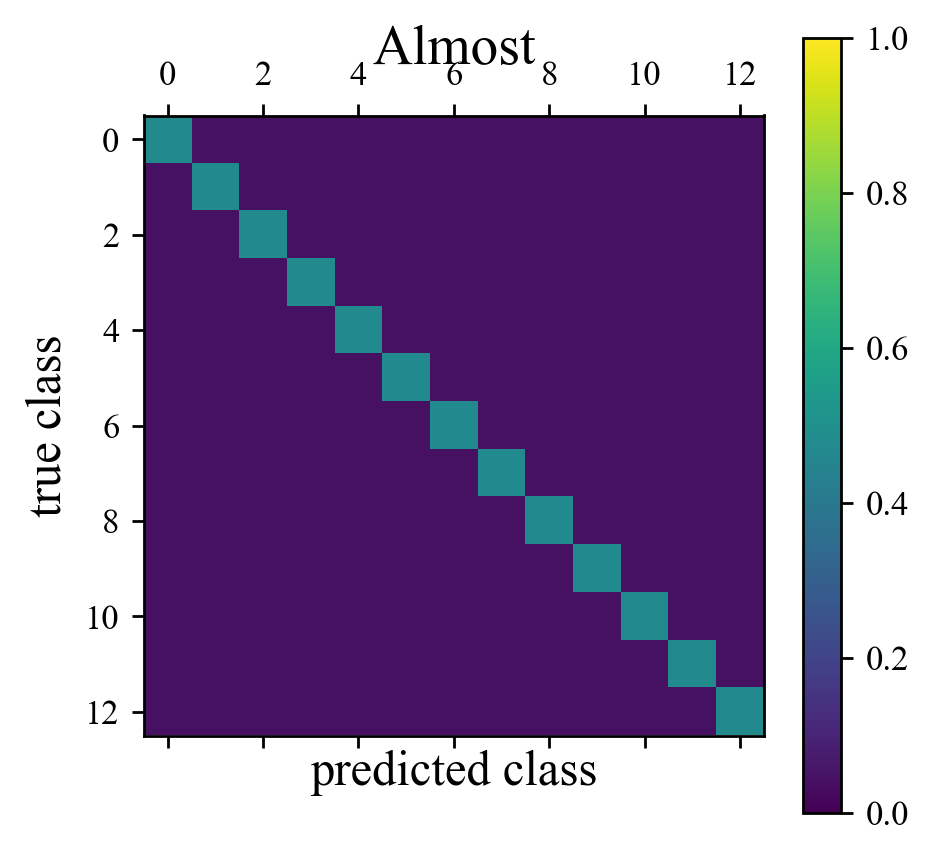
\includegraphics[width=0.45\textwidth]{./fig/Almost.png}\\
		\caption{}
		\label{fig:almost_data}
	\end{center}
\end{figure}

\subsubsection{Noisy classifier}
\label{sec:nois_datay}

a large perturbation of the perfect classifier

\begin{figure}
	\begin{center}
		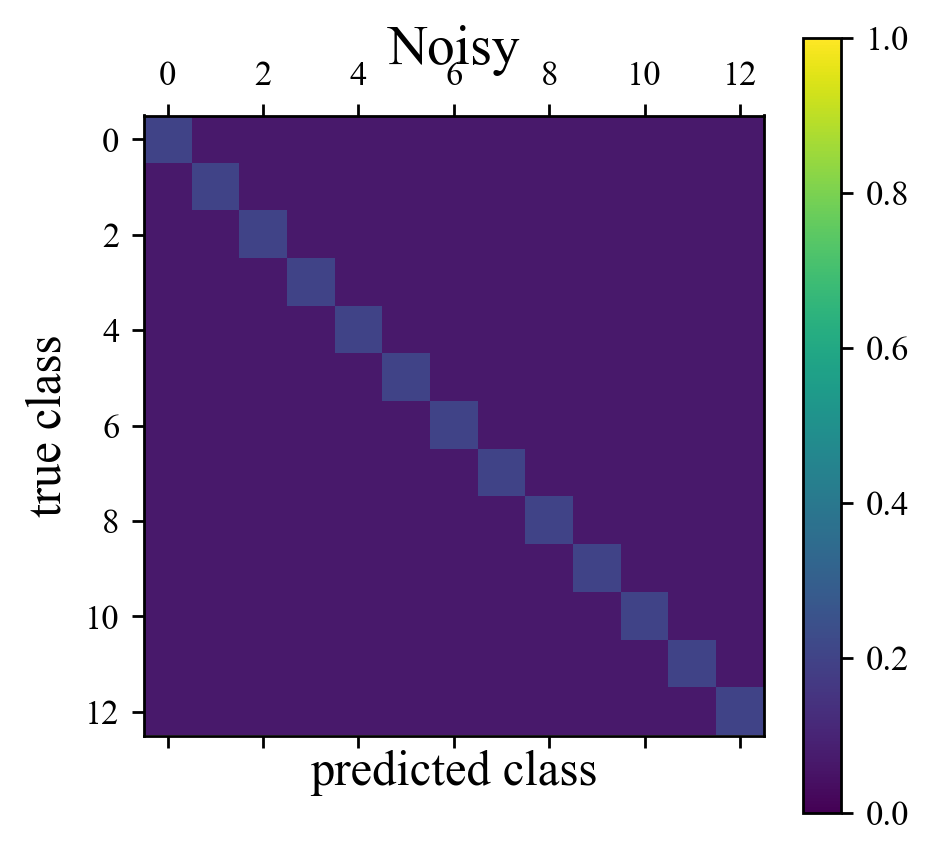
\includegraphics[width=0.45\textwidth]{./fig/Noisy.png}\\
		\caption{}
		\label{fig:noisy_data}
	\end{center}
\end{figure}

\subsubsection{Tunnel vision classifier}
\label{sec:tunnel_data}

classifies one class well and others randomly

\begin{figure}
	\begin{center}
		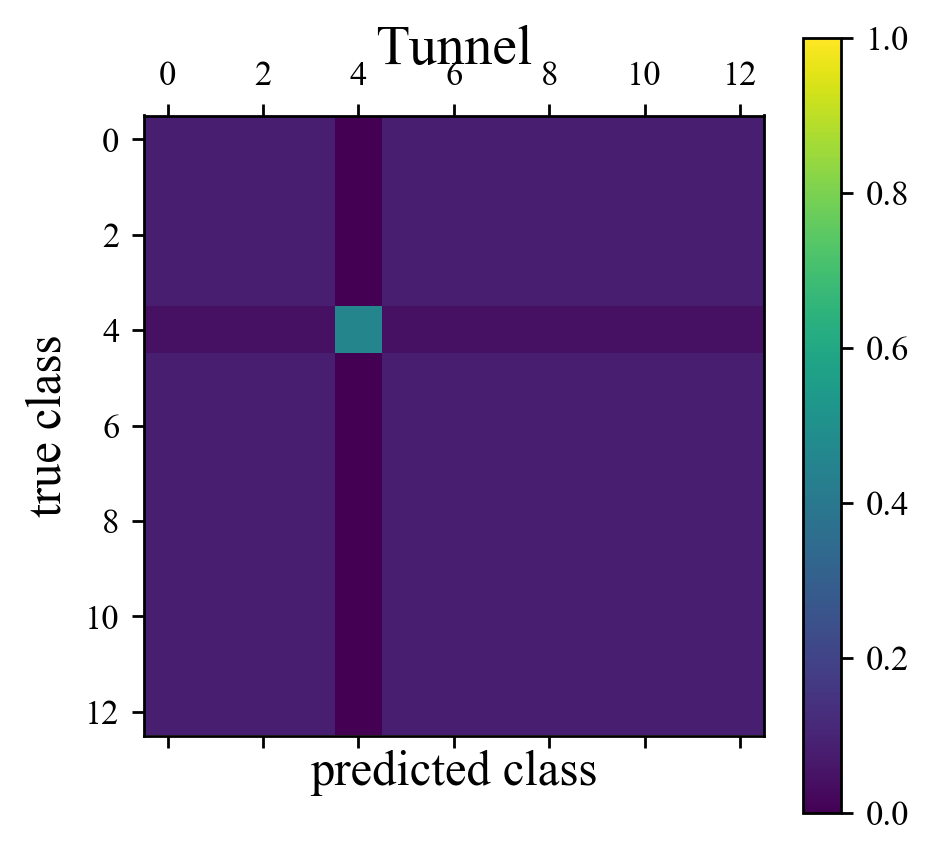
\includegraphics[width=0.45\textwidth]{./fig/Tunnel.png}\\
		\caption{}
		\label{fig:tunnel_data}
	\end{center}
\end{figure}

\subsubsection{Cruise control classifier}
\label{sec:cruise_data}

classifies all objects as a single class

\begin{figure}
	\begin{center}
		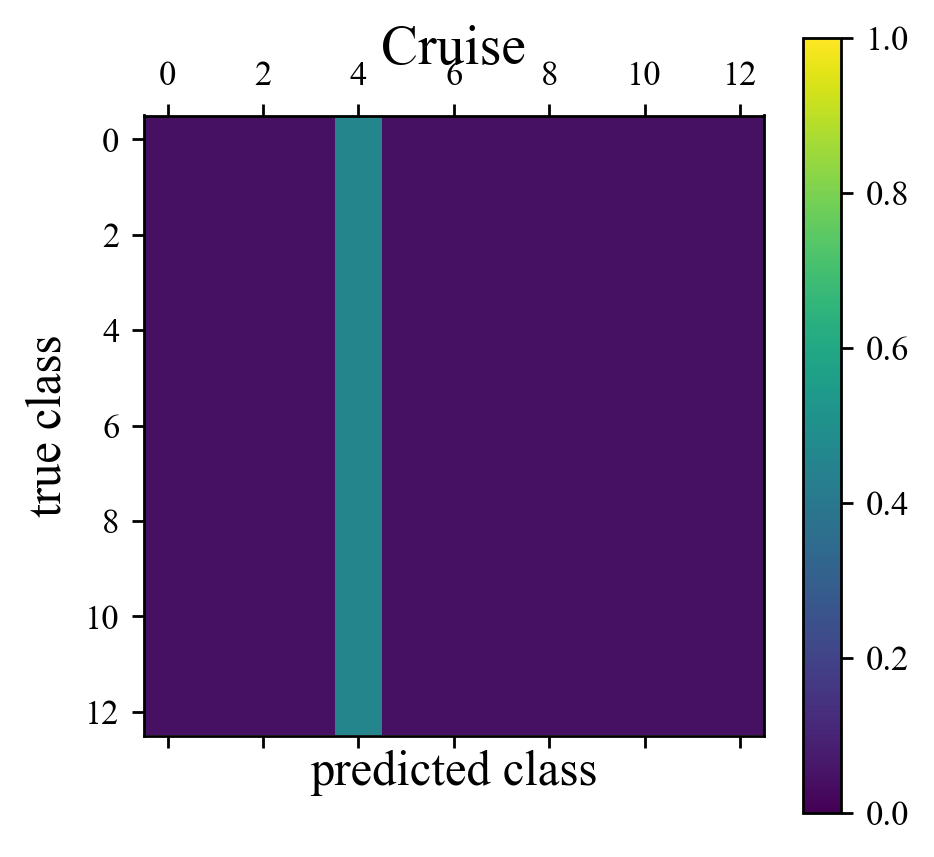
\includegraphics[width=0.45\textwidth]{./fig/Cruise.png}
		\caption{}
		\label{fig:cruise_data}
	\end{center}
\end{figure}

\subsubsection{Sumsuming classifier}
\label{sec:subsume_data}

consistently misclassifies one class as one other class

\begin{figure*}
	\begin{center}
		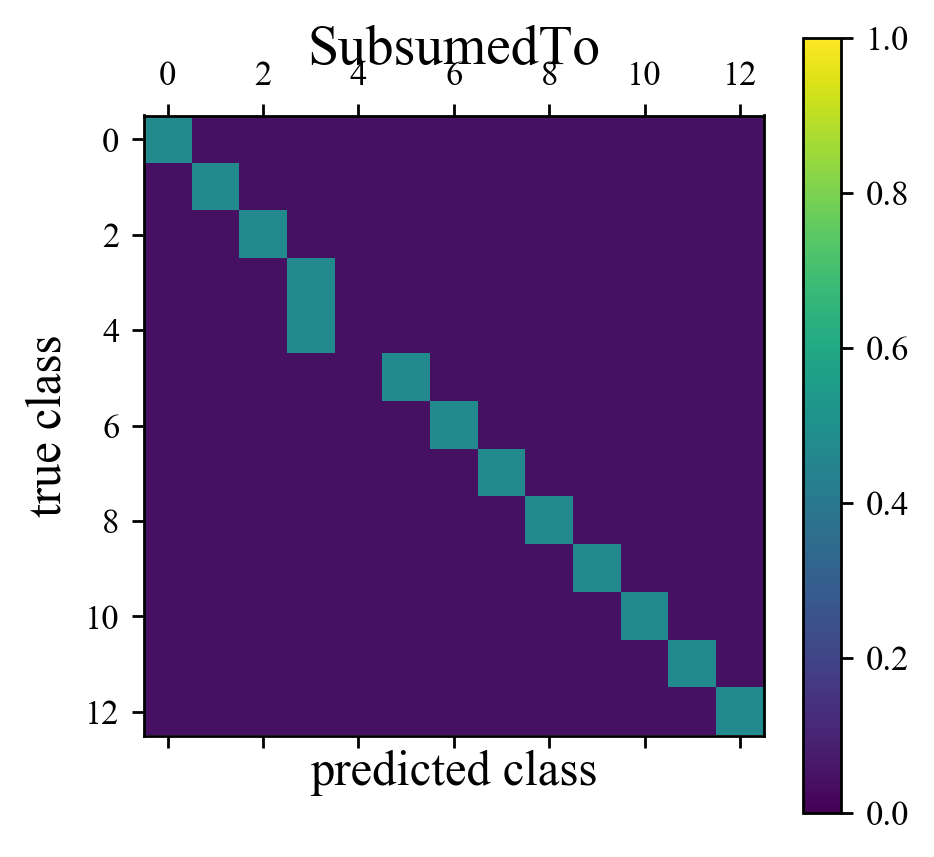
\includegraphics[width=0.45\textwidth]{./fig/SubsumedTo.png}
		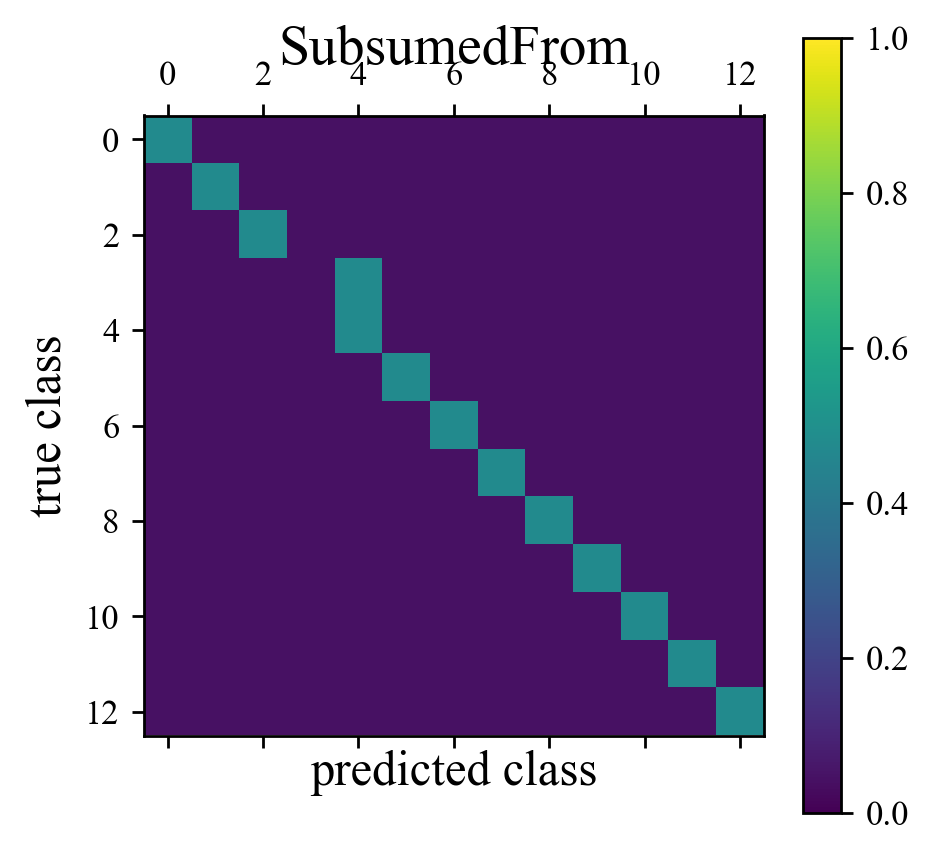
\includegraphics[width=0.45\textwidth]{./fig/SubsumedFrom.png}
		\caption{left: upweight the predicted class encompassing both true classes, right: upweight the predicted class that is consistently misclassified}
		\label{fig:subsume_data}
	\end{center}
\end{figure*}

\subsection{Representative classifications}
\label{sec:realdata}

\aim{Renee Hlozek will write the descriptions of these datasets.}

\aim{We should also do this for Ashish's data in the form of confusion matrices.}

\subsubsection{SNPhotCC}
\label{sec:snphotcc}

\begin{figure*}
	\begin{center}
		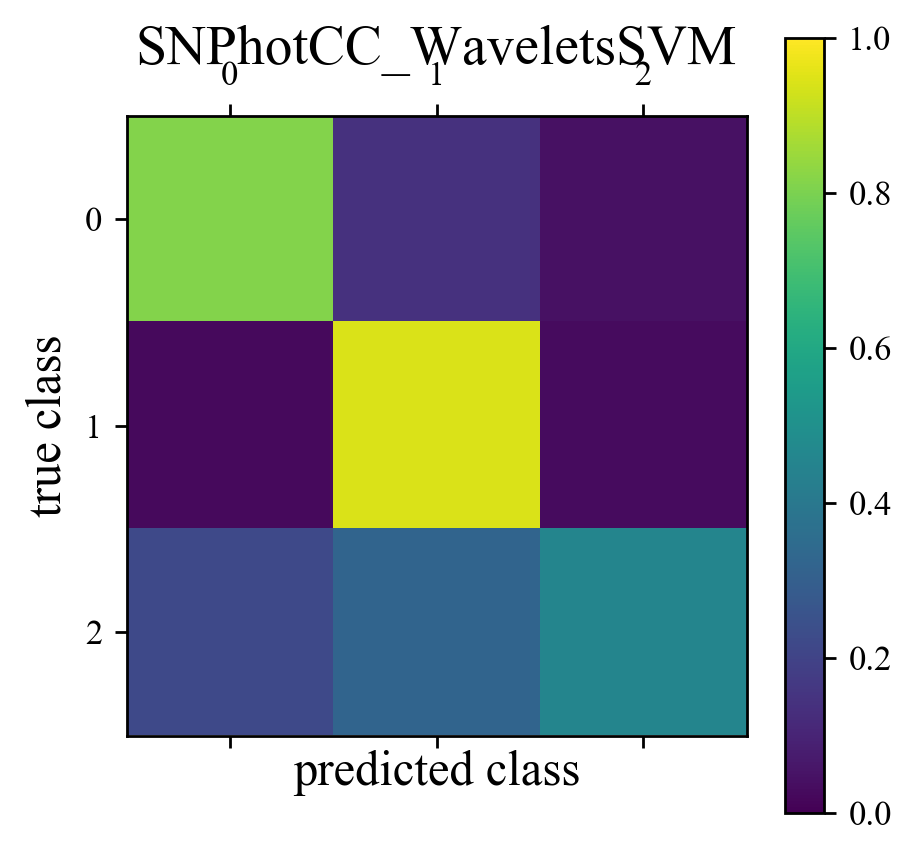
\includegraphics[width=0.24\textwidth]{./fig/SNPhotCC_WaveletsSVM_cm.png}
		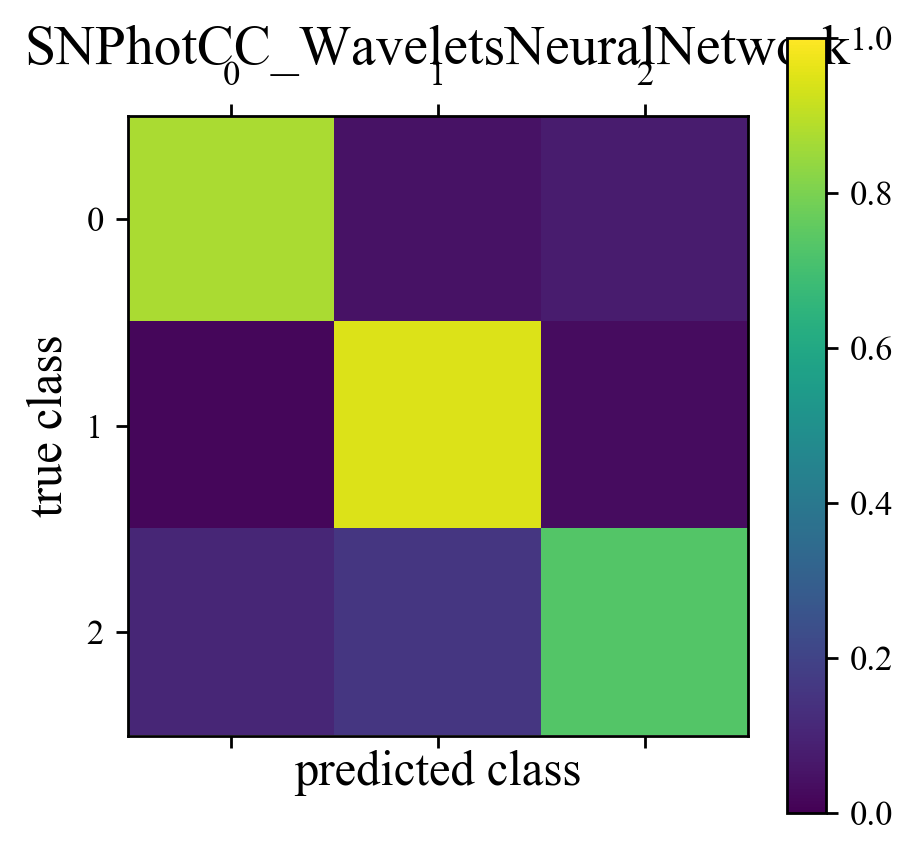
\includegraphics[width=0.24\textwidth]{./fig/SNPhotCC_WaveletsNeuralNetwork_cm.png}
		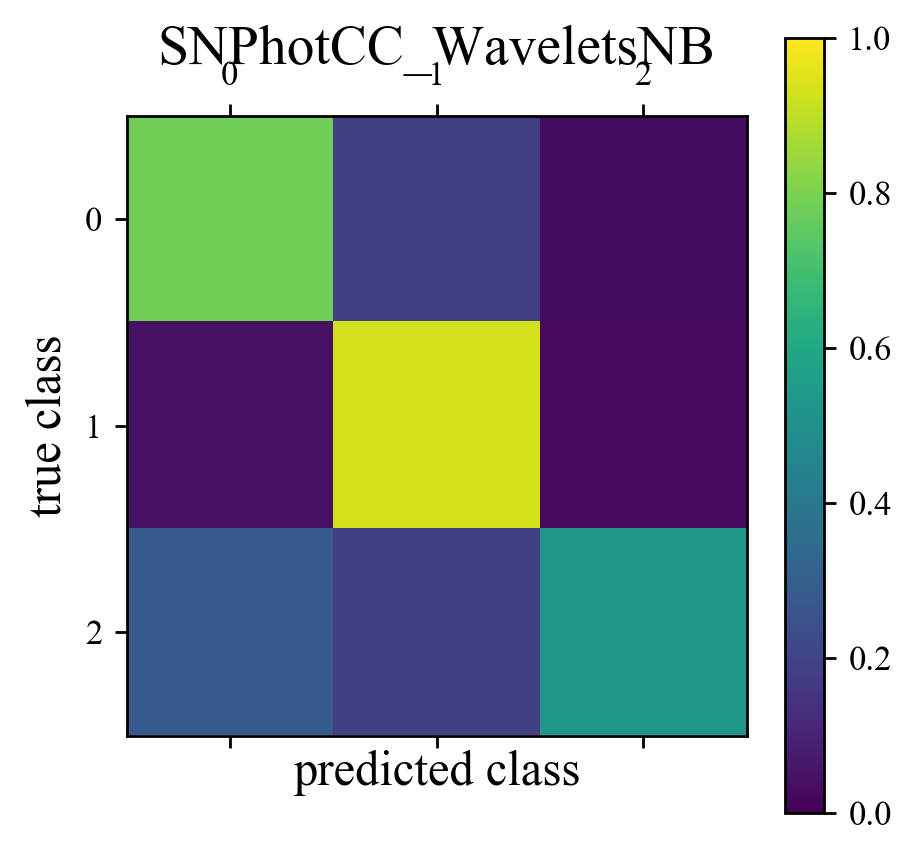
\includegraphics[width=0.24\textwidth]{./fig/SNPhotCC_WaveletsNB_cm.png}
		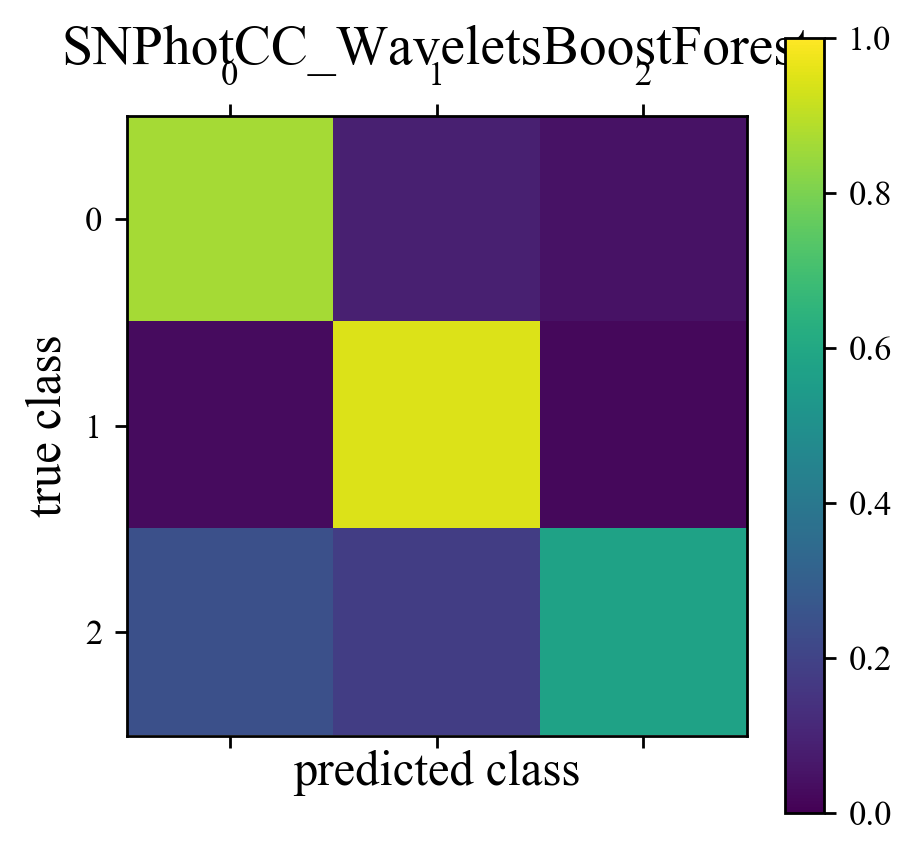
\includegraphics[width=0.24\textwidth]{./fig/SNPhotCC_WaveletsBoostForest_cm.png}\\
		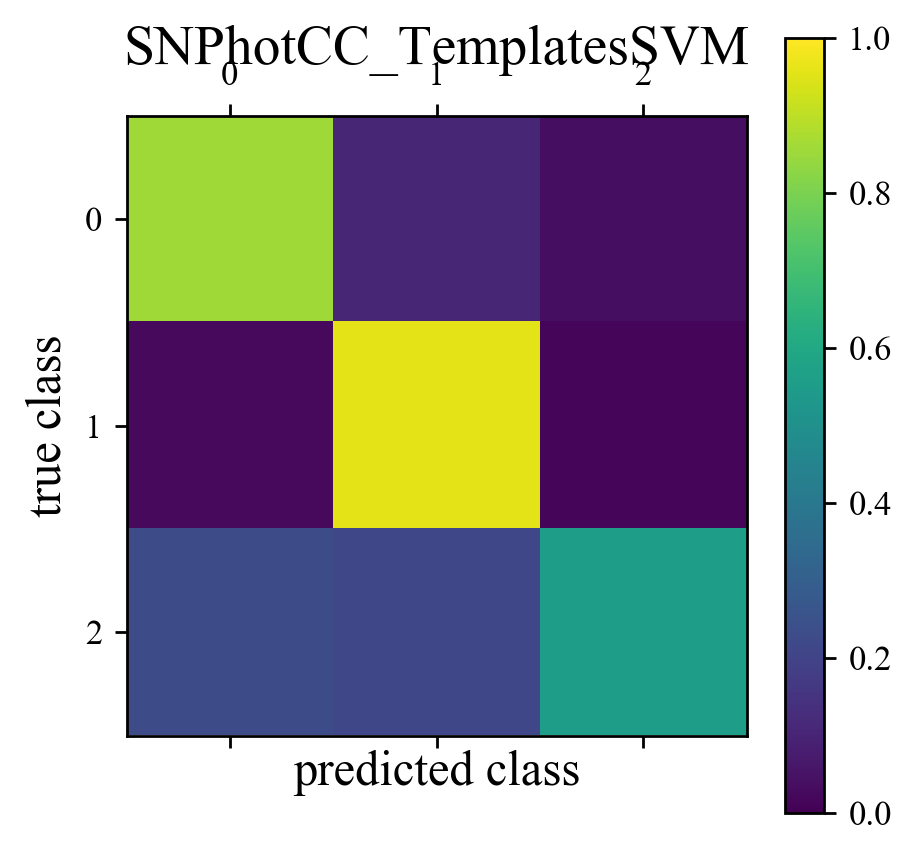
\includegraphics[width=0.24\textwidth]{./fig/SNPhotCC_TemplatesSVM_cm.png}
		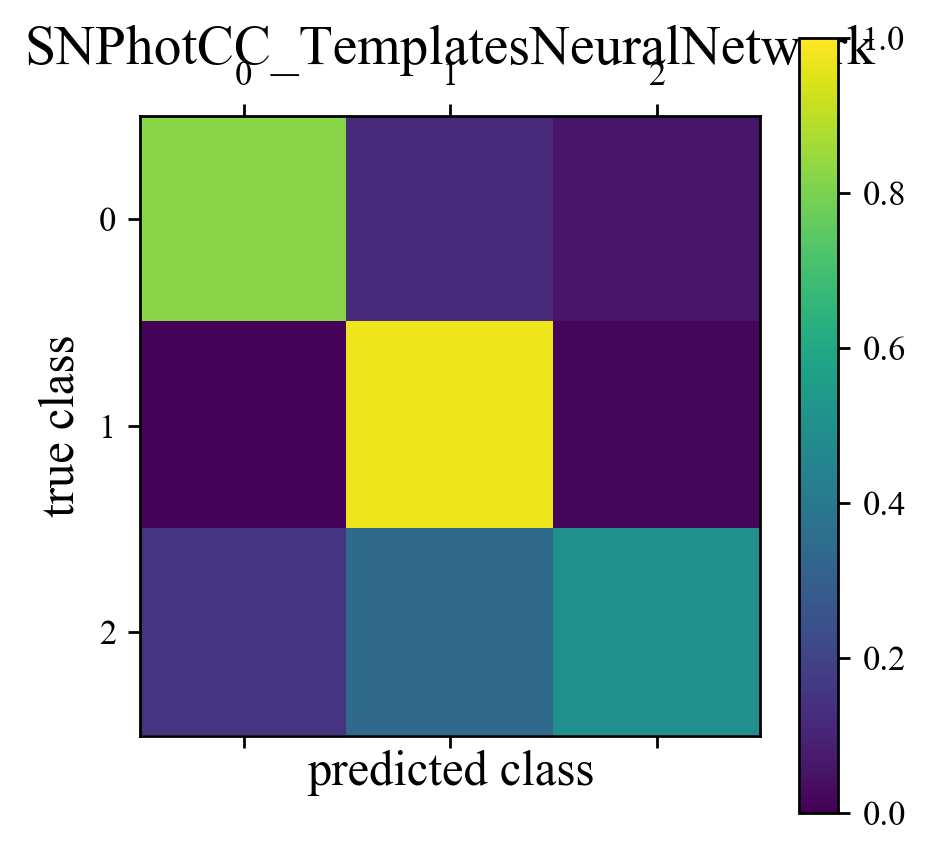
\includegraphics[width=0.24\textwidth]{./fig/SNPhotCC_TemplatesNeuralNetwork_cm.png}
		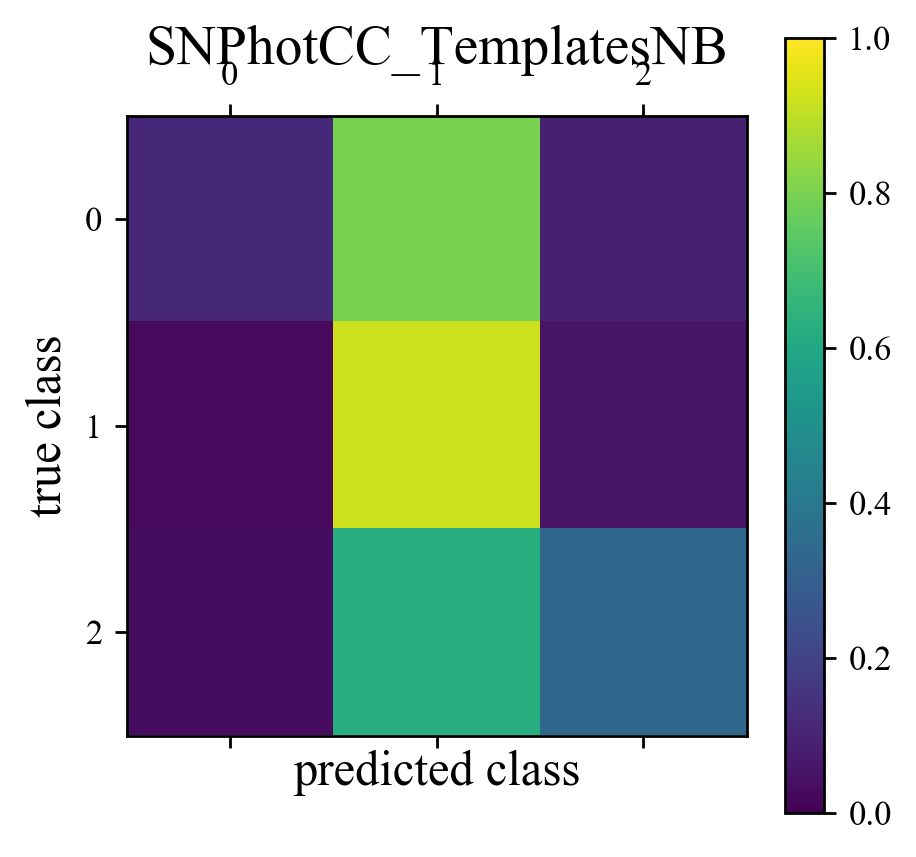
\includegraphics[width=0.24\textwidth]{./fig/SNPhotCC_TemplatesNB_cm.png}
		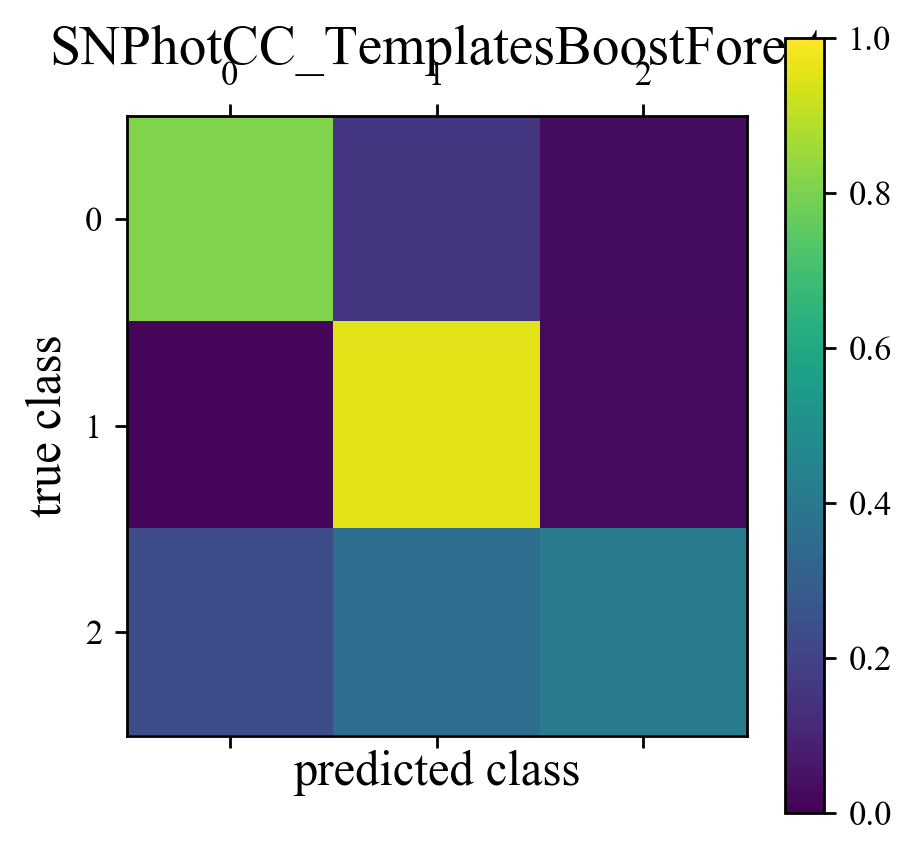
\includegraphics[width=0.24\textwidth]{./fig/SNPhotCC_TemplatesBoostForest_cm.png}
		\caption{}
		\label{fig:snphotcc_cm}
	\end{center}
\end{figure*}

\subsubsection{Unknown}
\label{sec:mystery}

\begin{figure*}
	\begin{center}
		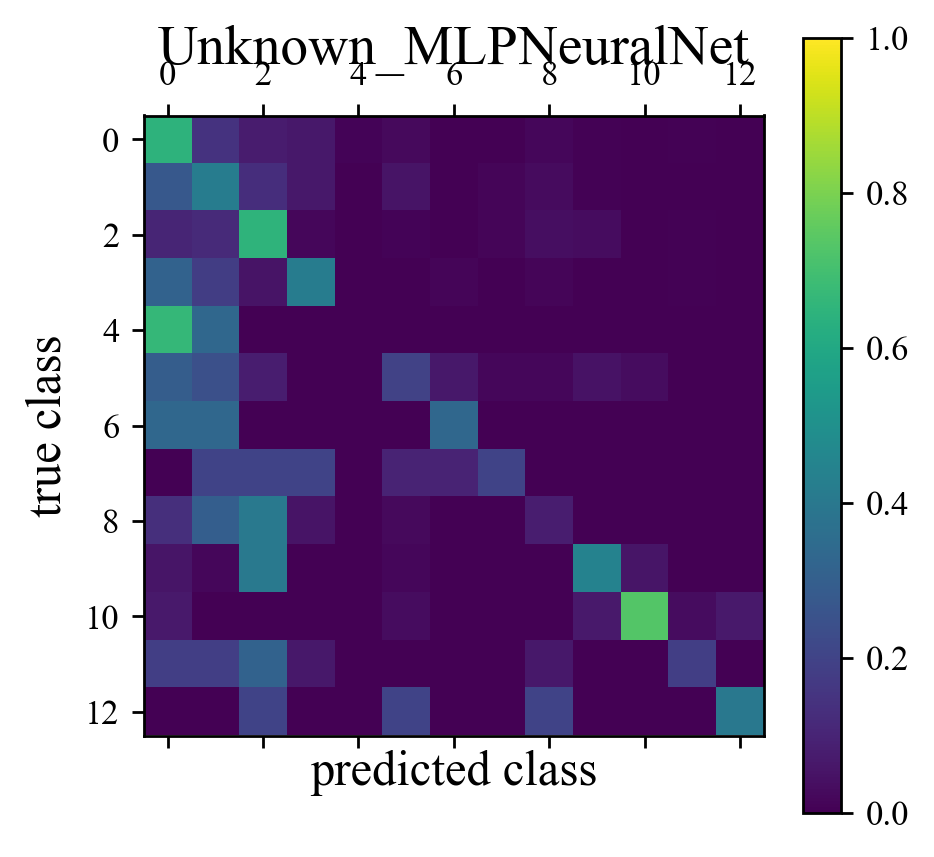
\includegraphics[width=0.3\textwidth]{./fig/Unknown_MLPNeuralNet_cm.png}
		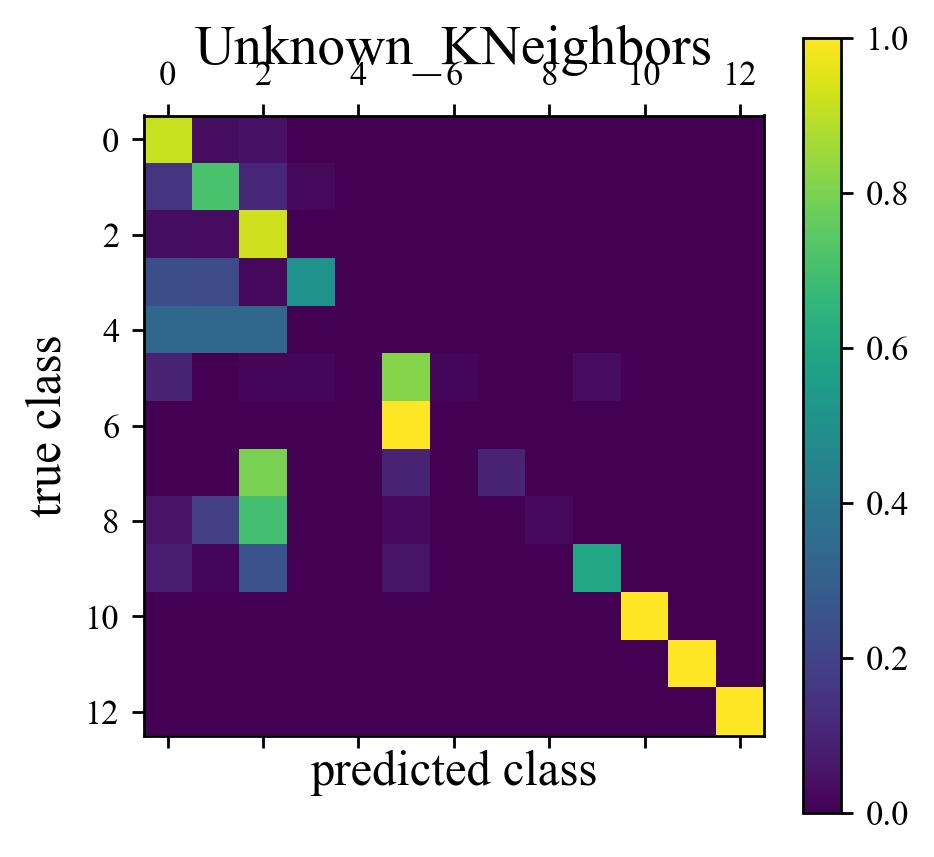
\includegraphics[width=0.3\textwidth]{./fig/Unknown_KNeighbors_cm.png}
		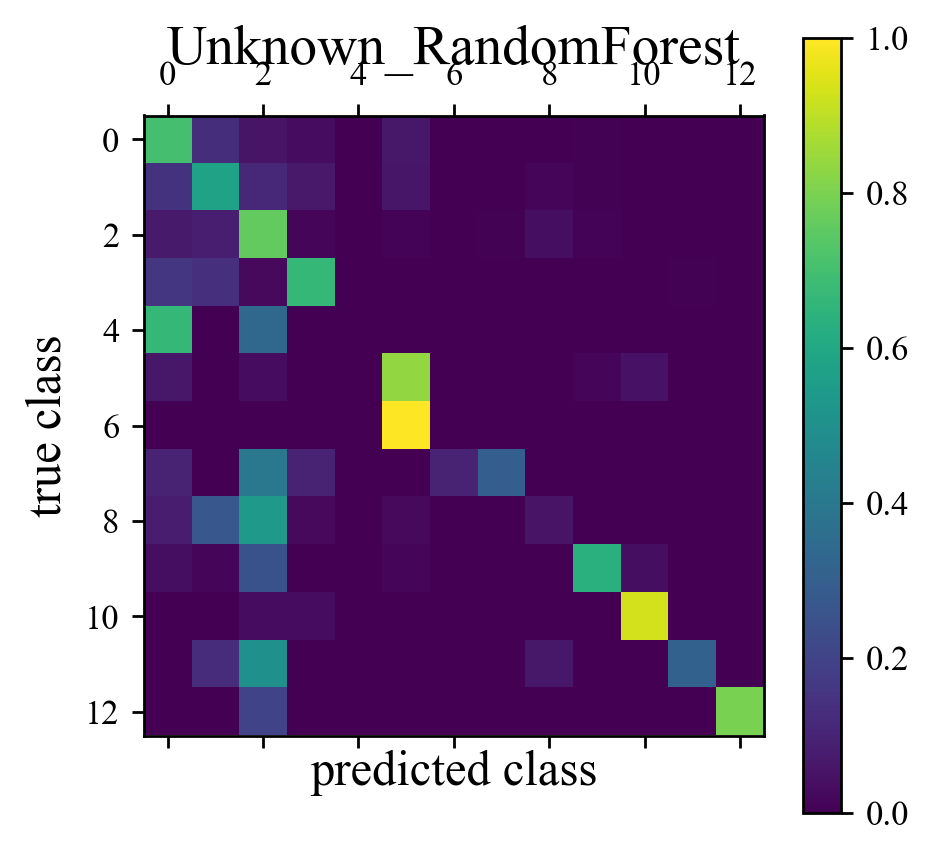
\includegraphics[width=0.3\textwidth]{./fig/Unknown_RandomForest_cm.png}
		\caption{}
		\label{fig:unknown_cm}
	\end{center}
\end{figure*}
